\documentclass[a4paper]{article}

\usepackage[francais]{babel}
\usepackage{amsmath}
\usepackage{amssymb}
\usepackage{graphicx}
%\usepackage{algorithmic}
\usepackage{url}
%\usepackage{subfig}
%\usepackage[squaren,Gray]{SIunits}

% reduce margin.
\usepackage[]{fullpage}

\makeatletter
\def\thickhrulefill{\leavevmode \leaders \hrule height 1pt\hfill \kern \z@}
\def\maketitle{
  \null
  \thispagestyle{empty}
  \vskip 1cm
  \begin{flushright}
	\normalfont\Large\@author
  \end{flushright}
  \vfil
  \hrule height 2pt
  \par
  \begin{center}
	\huge \strut \@title \par
  \end{center}
  \hrule height 2pt
  \par
  \vfil
  \vfil
  \null
\begin{center}
\end{center}
\begin{figure}[!ht]
	\centering
	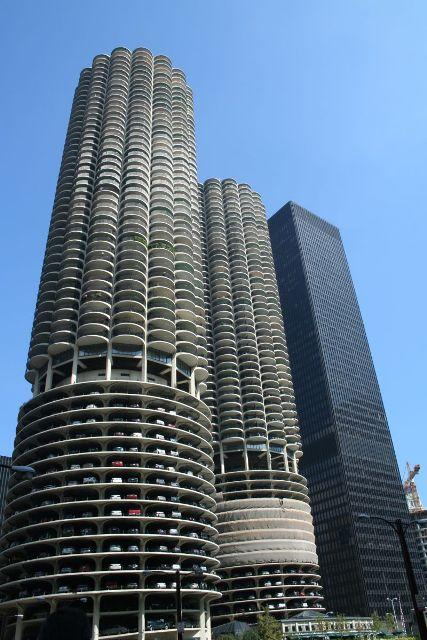
\includegraphics[scale=.5]{imgs/parkingpres.jpg}
\end{figure}
\begin{figure}[!ht]
	\centering
	
\includegraphics[scale=.5]{imgs/polytech.png}
\end{figure}
\vfil
  \cleardoublepage
  }
\makeatother
\author{Fran\c cois Chapuis, Roman Mkrtchian, K\'evin Rocher, Mathieu Bivert}
\title{Conception Objet: Mod\'elisation d'un parking \`a p\'eage}
\date{Ann\'ee scolaire $2011$-$2012$}

\begin{document}
\maketitle
\newpage
\tableofcontents
\newpage

\section{Pr\'esentation}
Ce document a pour but de r\'ealiser une mod\'elisation objet d'un parking \`a p\'eage.
Pour ce faire, on commencera par d\'ecrire de fa\c con g\'en\'erale le fonctionnement
du syst\`eme, pour ensuite rentrer dans les d\'etails via diff\'erents types de diagrammes
\'etudi\'es en cours\footnote{\url{http://users.polytech.unice.fr/~cm/}}.
\section{Description du syst\`eme}
Le parking, repr\'esent\'e figure \ref{parking}, est compos\'e de plusieurs entr\'ees,
sorties et caisses.
\begin{figure}[!ht]
	\centering
	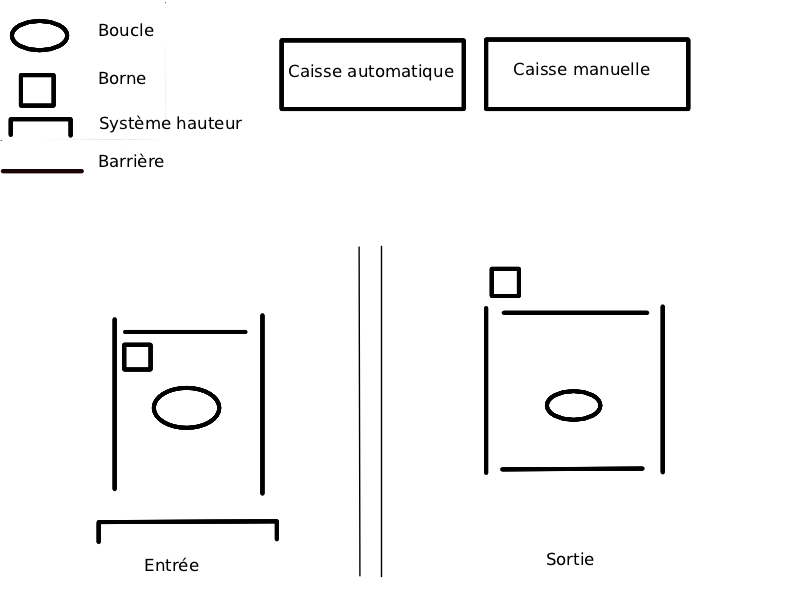
\includegraphics[scale=.7]{imgs/parking.png}
	\caption{\label{parking} Sch\'ema du parking. Pour simplifier, les \'el\'ements
		dupliqu\'es ne sont repr\'esent\'es qu'une seule fois}
\end{figure}

Une entr\'ee est typiquement constitu\'ee de :
\begin{description}
	\item[une boucle] au sol, permettant d'obtenir le poids magn\'etique du v\'ehicule
		passant dessus;
	\item[une barri\`ere] r\'egulant l'entr\'ee du parking;
	\item[une borne] compos\'ee d'un interphone, d'un distributeur de ticket et d'un
		lecteur de cartes;
	\item[un syst\`eme de limitation en hauteur], afin de refuser l'entr\'ee aux
		v\'ehicules trop imposants.
\end{description}

La borne situ\'ee \`a l'entr\'ee permet soit d'obtenir un ticket magn\'etique, soit de
prendre l'empreinte d'une carte bancaire ou encore d'une carte d'abonnement. Ce sont,
comme on le verra plus tard, les trois grands moyens de payements mis en \o euvre. De
plus, la pr\'esence d'un interphone permet de contacter un employ\'e du parking en
cas de besoin.

Une sortie a une composition similaire \`a celle d'une entr\'ee, au d\'etail pr\`es
qu'elle dispose de deux barri\`eres, et que le syst\`eme de limitation en hauteur
lui a \'et\'e retir\'e.

On distingue deux types de caisses: les caisses automatiques ainsi qu'une caisse
manuelle.

\subsection{Acteurs}
On identifie plusieurs acteurs pouvant int\'eragir au niveau du parking:
\begin{itemize}
	\item Le client;
	\item le surveillant du parking;
	\item le technicien;
	\item la banque;
	\item la fourri\`ere;
	\item la soci\'et\'e g\'erant le parking.
\end{itemize}

\subsubsection{Client}
Les clients sont class\'es en trois cat\'egories, selon la fa\c con qu'ils ont choisie
pour rentrer dans le parking, \`a savoir:
\begin{itemize}
	\item les clients abonn\'es, utilisant une carte d'abonnement;
	\item les clients rentrant \`a l'aide d'une carte bancaire;
	\item les autres clients, c'est \`a dire ceux qui ont r\'ecup\'er\'e un
		ticket magn\'etique.
\end{itemize}
\subsubsection{Surveillant du parking}
Il est charg\'e de v\'erifier et d'approvisionner les bornes ainsi que les caisses
de payements en consommables (papier, monnaie, $\hdots$). C'est \`a lui que les
clients vont parler lorsqu'ils d\'ecident d'utiliser un des interphones situ\'es sur
les bornes. De plus, c'est l'acteur charg\'e de communiquer au technicien les \'eventuelles
d\'efaillances techniques, ou encore de pr\'evenir la fourri\`ere en cas de stationnement
prolong\'e d'un v\'ehicule.

Enfin, le surveillant est charg\'e de s'occuper de la caisse manuelle.

\subsubsection{Technicien}
C'est \`a lui qu'incombe la t\^ache de v\'erifier et d'entretenir les diff\'erents
composants du parking (barri\`ere, borne, $\hdots$). Il est pr\'evenu par le surveillant
en cas de probl\`eme. 

Selon la taille du parking et les besoins de la soci\'et\'e de parking, les r\^oles
de surveillant et de technicien peuvent bien entendu \^etre occup\'es par la m\^eme
personne.

\subsubsection{Banque}
\`A la fin de la journ\'ee, toutes les transactions bancaires lui sont envoy\'ees. Elle
a pour r\^ole de les r\'ecuperer et de le traiter.

\subsubsection{Fourri\`ere}
Si un v\'ehicule est stationn\'e sur le parking depuis au moins $72$ heures dans l'enceinte
du parking, la fourri\`ere a de fortes chances d'\^etre appell\'ee par le surveillant afin
de venir r\'ecuperer le v\'ehicule.

\subsubsection{Soci\'et\'e de parking}
C'est elle qui poss\`ede et g\`ere le parking. Elle intervient ici essentiellement pour
recevoir les statistiques sur l'utilisation du parking, envoy\'e une fois par jour, au
m\^eme moment que les transactions bancaires.

\subsection{Fonctionnalit\'es}
Les acteurs vont int\'eragir sur le syst\`eme au travers de deux grandes fonctionnalit\'es:
\begin{enumerate}
	\item \textit{Se garer};
	\item \textit{Gestion du parking}.
\end{enumerate}

XXX

Les sc\'enarios Cokburn donnent une description plus pr\'ecise et compl\`ete des diff\'erents
\'elements de ces fonctionnalit\'es.

\section{Diagrammes des cas d'utilisation (Use case)}
\section{Sc\'enarios Cockburn}
\subsection{Se garer}
\begin{description}
	\item[Cas d'utilisation] se garer
	\item[Acteur primaire] client
	\item[Acteur support] surveillant
	\item[Pr\'econdition] place libre dans le parking
	\item[Sc\'enario Primaire] \
	\begin{enumerate}
		\item Le client passe sous le syst\`eme de d\'etection de hauteur;
		\item le client passe sur la boucle;
		\item le client demande un ticket;
		\item le client prend son ticket;
		\item la barri\`ere se l\`eve;
		\item le client rentre;
		\item la barri\`ere se referme;
		\item le client se garre;
		\item le client introduit son ticket d'entr\'ee dans la borne de payement;
		\item \textbf{le client paye};
		\item le client re\c coit son ticket de sortie;
		\item le client introduit le ticket de sortie dans la borne de sortie;
		\item la premi\`ere barri\`ere de sortie se l\`eve;
		\item le client s'avance sur la boucle;
		\item la premi\`ere barri\`ere de sortie se referme;
		\item la seconde barri\`ere de sortie se l\`eve;
		\item le client sort;
		\item la deuxi\`eme barri\`ere s'abaisse.
	\end{enumerate}
	\item[Postcondition] le client s'est garr\'e et est sortit du parking
	\item[Variantes] \
\end{description}

\subsection{Gestion du parking}
\begin{description}
	\item[Cas d'utilisation] gestion du parking
	\item[Acteur primaire] le syst\`eme
	\item[Acteur support]  la fourri\`ere, le surveillant, le technicien, soci\'et\'e
				de parking
	\item[Pr\'econdition] 
	\item[Sc\'enario Primaire] \
	\begin{enumerate}
		\item Le surveillant appelle la fourri\`ere si un v\'ehicule est
		pr\'esent sur le parking depuis plus de $72$ heures;
		\item le surveillant appelle le technicien en cas de probl\`emes
		techniques sur le parking;
		\item le technicien maintient r\'eguli\`erement les diff\'erents
		\'el\'ements du parking;
		\item le surveillant s'occupe d'alimenter les machines en consommables
		lorsque celles-ci lui signale un manque;
		\item le surveillant alimente r\'eguli\`erement les caisses en
		monnaie et les bornes en consommables;
		\item le syst\`eme envoie quotidiennement \`a la soci\'et\'e des
		informations relatives aux clients (dans le but d'\'etablir des
		statistiques);
		\item le syst\`eme envoie quotidiennement \`a la soci\'et\'e les
		diff\'erentes transactions bancaires \`a effectuer.
	\end{enumerate}
	\item[Postcondition] les probl\`emes, s'il y en a, sont r\'esolus
	\item[Variantes] \
\end{description}

\subsection{Payer}
\begin{description}
	\item[Cas d'utilisation] payer
	\item[Acteur primaire] le client
	\item[Acteur support]  
	\item[Pr\'econdition] 
	\item[Sc\'enario Primaire] \
	\item[Postcondition] les probl\`emes, s'il y en a, sont r\'esolus
	\item[Variantes] \
\end{description}

\section{Diagrammes d'activit\'es}

\end{document}
